\section{CHARACTER DETECTION}

For the last endeavor of this project, we are to detect and predict letters in an image with the help of object detection or object localization. We were able to do so with the help of our classifiers and a technique called \textit{sliding window}. The idea behind a sliding window is to divide a larger image into smaller windows of fixed size and apply an image classifier to determine if a target is in the picture - in our case a letter. We implemented a simple adjustable sliding window for each of the algorithms, which returns an image with green squares around a \textit{valid} classification while printing the letter.

\subsection{Detection}
% Test your character detector on detection-1.jpg and detection-2.jpg and show the result in the report.  Feel free to find or create additional images to test your detector, if you are so inclined.
The parameters for the following two detection images were kept the same: the step size was kept at 4, i.e. it moves 4 pixels per window, and the window size was 20x20.

\subsubsection{detection-1.jpg}
Both methods were capable of detecting all letters, but apparently struggled with the 'S' . The sliding windows whose classification had a confidence level higher than the probability threshold set in the algorithm are shown as green squares in Figure \ref{fig:svm_detect}. To be able to classify the 'S', the confidence boundary of both algorithms were reduced to \textasciitilde 88\%, which is why a second 'E' is classified (if you look closely).

\begin{figure}[H]
    \centering
    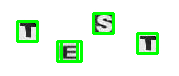
\includegraphics[width=0.2\textwidth]{pictures/svm_pred.png}
    \caption{"T-E-S-T"}
    \label{fig:svm_detect}
\end{figure}

\subsubsection{detection-2.jpg}

The second image (figure \ref{fig:svm_detect2}) was predicted by the CNN model. The performance was not satisfactory at all and there are a few things we could have done differently, which will be discussed in the evaluation of this section. There seemed to be a problem with the confidence of our Keras CNN models, as it was almost always above 99.9\% sure about its classifications, which made it hard to decide on a confidence threshold and partly explains all the redundant squares. The model had ~65\% accuracy in the classifications made in the image.


\begin{figure}[H]
    \centering
    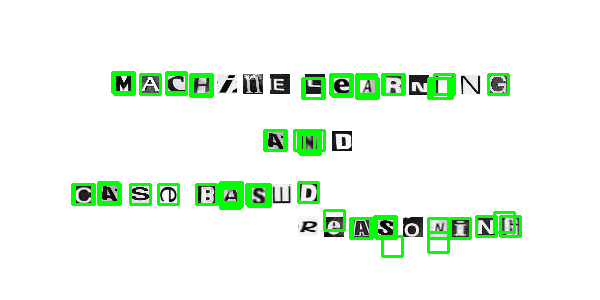
\includegraphics[width=0.5\textwidth]{pictures/svm_pred2.png}
    \caption{"MACHINE LEARNING AND CASE BASED REASONING"}
    \label{fig:svm_detect2}
\end{figure}

\subsection{Evaluation and potential improvements}
% Give an evaluation of your detection system.  How does it perform?
% Describe any improvements you made to your detector.  Discuss how you can improve your system further.

Our detection algorithms performed well on the first image and not so good on the second, but it has a lot of potential. The first giveaway is that the required confidence level that were used could be lower in order to detect the more obscure letters. We could have reduced it if we implemented a restriction to the re-classification of the same letters in windows close to each other. A simple votation or average confidence between of the neighboring windows was considered, as well as removing outliers such as all-white images. An average of neighbors would also reduce the possibility of a faulty classification.

Another improvement we could have tried is to use different representations of the image and the sliding windows. Characters could have different orientations, and different angles and projections of the image/window should be evaluated and consider as possible classifications. 

Every possible scale of the image could also be considered. One possible way to do this is to use "\textit{Image Pyramids}", which is a multi-scale representation of an image. This would help our sliding window by making it able to classify characters that require smaller scales.

In the second detection image (figure \ref{fig:svm_detect2}) there was a lot more obscure characters and some with different orientations. As we mentioned, this could have been accounted for if we had extended our dataset with augmented representations of the existing samples.
